\documentclass[svgnames,table,,aspectratio=169]{beamer}
%\documentclass[svgnames,table,handout,aspectratio=129]{beamer}
\usepackage{hhline}
\usepackage{etoolbox}
\usepackage{tikz}
%\usepackage{tikz-3dplot}
\usepackage{mathtools}
\usepackage{amssymb}
%\usepackage{/usr/lib64/R/share/texmf/Sweave}
\usepackage{polynom}
\usepackage{qrcode}


%\input{latexdefinitions}
\definecolor{georgiaRed}{RGB}{100,0,00}
\definecolor{mediumGray}{gray}{0.6}



\usetheme{Frankfurt}%
%\usetheme{Warsaw}%
%\useoutertheme{smoothbars}


%\usecolortheme{seagull}
\usecolortheme{beaver}
\logo{\includegraphics[height=.125in]{ugaLogo}}

% Note that the colour definitions are given in the latexDefinitions
% file.
\setbeamercolor{palette primary}{fg=georgiaRed,bg=white}
\setbeamercolor{palette secondary}{fg=georgiaRed,bg=white}
\setbeamercolor{palette tertiary}{fg=georgiaRed,bg=white}
\setbeamercolor{palette quaternary}{bg=mediumGray,fg=black}
\setbeamercolor{block title}{fg=black,bg=black!15}
\setbeamercolor{block body}{fg=black,bg=black!10}
\setbeamercolor{titlelike}{bg=georgiaRed,fg=white} % parent=palette quaternary}

\setbeamercolor{block title}{fg=white,bg=georgiaRed}
\setbeamercolor{block body}{parent=normal text,use=block title,bg=black!5!white}

% Define the variable to determine whether or not the clicker quizzes
% are visible in the resulting output.
\newtoggle{clicker}
\toggletrue{clicker}
%\togglefalse{clicker}


% To display a lecture uncomment out the "includeonly" line below to
% match the name of the file. You do not have to do anything with the
% lecture line below and can leave it commented out. It is in place
% because at one time we had multiple lectures within a file, but that
% has been changed.



\mode<presentation>{
  \setbeamercovered{invisible}
  \setbeameroption{hide notes}
}

\mode<handout>{
 
  \usepackage{pgfpages}
  %\pgfpagesuselayout{4 on 1}[letterpaper, border shrink=5mm]
  \pgfpagesuselayout{resize to}[letterpaper,border shrink=5mm]
  \setbeameroption{show notes}


  %\pgfpagesphysicalpageoptions{logical pages=2,physical
  %height=\pgfpageoptionheight,physical width=\pgfpageoptionwidth}
  % Set up the pages for notes.
  % This idea and some code came from
  % http://www.guidodiepen.nl/2009/07/creating-latex-beamer-handouts-with-notes/



  \pgfpagesdeclarelayout{3 on 1 with notes} {
    \edef\pgfpageoptionheight{11in} %\the\paperheight}
    \edef\pgfpageoptionwidth{8.5in} %\the\paperwidth}
    \edef\pgfpageoptionborder{0pt}
  }

  {

	\AtBeginDocument{
      \newbox\notesbox
      \setbox\notesbox=\vbox{
        \hsize=\paperwidth
        \vskip-2.5cm\hskip-5cm\vbox{
          \textcolor{light-gray}{\hrule width 12.6cm\vskip0.5cm}
          \textcolor{light-gray}{\hrule width 12.6cm\vskip0.5cm}
          \textcolor{light-gray}{\hrule width 12.6cm\vskip0.5cm}
          \textcolor{light-gray}{\hrule width 12.6cm\vskip0.5cm}
          \textcolor{light-gray}{\hrule width 12.6cm\vskip0.5cm}
          \textcolor{light-gray}{\hrule width 12.6cm\vskip0.5cm}
          \textcolor{light-gray}{\hrule width 12.6cm\vskip0.5cm}
          \textcolor{light-gray}{\hrule width 12.6cm\vskip0.5cm}
          \textcolor{light-gray}{\hrule width 12.6cm\vskip0.5cm}
          \textcolor{light-gray}{\hrule width 12.6cm\vskip0.5cm}
          \textcolor{light-gray}{\hrule width 12.6cm\vskip0.5cm}
          \textcolor{light-gray}{\hrule width 12.6cm\vskip0.5cm}
          \textcolor{light-gray}{\hrule width 12.6cm\vskip0.5cm}
          \textcolor{light-gray}{\hrule width 12.6cm\vskip0.5cm}
          \textcolor{light-gray}{\hrule width 12.6cm\vskip0.5cm}
          \textcolor{light-gray}{\hrule width 12.6cm\vskip0.5cm}
          \textcolor{light-gray}{\hrule width 12.6cm\vskip0.5cm}
          \textcolor{light-gray}{\hrule width 12.6cm\vskip0.5cm}
          \textcolor{light-gray}{\hrule width 12.6cm\vskip0.5cm}

          \vspace*{-9.75cm}
          \textcolor{light-gray}{\rule[-1.0cm]{1pt}{9.25cm}\hskip0.5cm}
          \textcolor{light-gray}{\rule[-1.0cm]{1pt}{9.25cm}\hskip0.5cm}
          \textcolor{light-gray}{\rule[-1.0cm]{1pt}{9.25cm}\hskip0.5cm}
          \textcolor{light-gray}{\rule[-1.0cm]{1pt}{9.25cm}\hskip0.5cm}
          \textcolor{light-gray}{\rule[-1.0cm]{1pt}{9.25cm}\hskip0.5cm}
          \textcolor{light-gray}{\rule[-1.0cm]{1pt}{9.25cm}\hskip0.5cm}
          \textcolor{light-gray}{\rule[-1.0cm]{1pt}{9.25cm}\hskip0.5cm}
          \textcolor{light-gray}{\rule[-1.0cm]{1pt}{9.25cm}\hskip0.5cm}
          \textcolor{light-gray}{\rule[-1.0cm]{1pt}{9.25cm}\hskip0.5cm}
          \textcolor{light-gray}{\rule[-1.0cm]{1pt}{9.25cm}\hskip0.5cm}
          \textcolor{light-gray}{\rule[-1.0cm]{1pt}{9.25cm}\hskip0.5cm}
          \textcolor{light-gray}{\rule[-1.0cm]{1pt}{9.25cm}\hskip0.5cm}
          \textcolor{light-gray}{\rule[-1.0cm]{1pt}{9.25cm}\hskip0.5cm}
          \textcolor{light-gray}{\rule[-1.0cm]{1pt}{9.25cm}\hskip0.5cm}
          \textcolor{light-gray}{\rule[-1.0cm]{1pt}{9.25cm}\hskip0.5cm}
          \textcolor{light-gray}{\rule[-1.0cm]{1pt}{9.25cm}\hskip0.5cm}
          \textcolor{light-gray}{\rule[-1.0cm]{1pt}{9.25cm}\hskip0.5cm}
          \textcolor{light-gray}{\rule[-1.0cm]{1pt}{9.25cm}\hskip0.5cm}
          \textcolor{light-gray}{\rule[-1.0cm]{1pt}{9.25cm}\hskip0.5cm}
          \textcolor{light-gray}{\rule[-1.0cm]{1pt}{9.25cm}\hskip0.5cm}

        }

      }

    \pgfpagesphysicalpageoptions
    {%
      logical pages=6,%
      physical height=\pgfpageoptionheight,%
      physical width=\pgfpageoptionwidth,%
      last logical shipout=3%
    }
    
    \pgfpageslogicalpageoptions{1}
    {%
      border shrink=\pgfpageoptionborder,%
      resized width=.5\pgfphysicalwidth,%
      resized height=.33\pgfphysicalheight,%
      center=\pgfpoint{.25\pgfphysicalwidth}{.82\pgfphysicalheight}%
    }%
    \pgfpageslogicalpageoptions{2}
    {%
      border shrink=\pgfpageoptionborder,%
      resized width=.5\pgfphysicalwidth,%
      resized height=.33\pgfphysicalheight,%
      center=\pgfpoint{.25\pgfphysicalwidth}{.47\pgfphysicalheight}%
    }%
    \pgfpageslogicalpageoptions{3}
    {%
      border shrink=\pgfpageoptionborder,%
      resized width=.5\pgfphysicalwidth,%
      resized height=.33\pgfphysicalheight,%
      center=\pgfpoint{.25\pgfphysicalwidth}{.17\pgfphysicalheight}%
    }%	
	\pgfpageslogicalpageoptions{4}
    {%
      border shrink=\pgfpageoptionborder,%
      resized width=.5\pgfphysicalwidth,%
      resized height=.33\pgfphysicalheight,%
      center=\pgfpoint{.85\pgfphysicalwidth}{.82\pgfphysicalheight},%
      copy from=4
    }%
    \pgfpageslogicalpageoptions{5}
    {%
      border shrink=\pgfpageoptionborder,%
      resized width=.5\pgfphysicalwidth,%
      resized height=.33\pgfphysicalheight,%
      center=\pgfpoint{.85\pgfphysicalwidth}{.47\pgfphysicalheight},%
      copy from=5
    }%
    \pgfpageslogicalpageoptions{6}
    {%
      border shrink=\pgfpageoptionborder,%
      resized width=.5\pgfphysicalwidth,%
      resized height=.33\pgfphysicalheight,%
      center=\pgfpoint{.85\pgfphysicalwidth}{.17\pgfphysicalheight},%
      copy from=6
    }%
    
      \pgfpagesshipoutlogicalpage{4}\copy\notesbox
      \pgfpagesshipoutlogicalpage{5}\copy\notesbox
      \pgfpagesshipoutlogicalpage{6}\copy\notesbox
    }
  }

  \pgfpagesuselayout{3 on 1 with notes}

}

\setbeamercolor{upper separation line head}{bg=red}
\setbeamercolor{headline}{bg=red}
\setbeamertemplate{headline}
{%
\begin{beamercolorbox}{section in head/foot}
\insertsectionnavigationhorizontal{.75\textwidth}{}{}
\hfill \insertpagenumber /\insertdocumentendpage
\end{beamercolorbox}%
}
\setbeamercolor{section number projected}{bg=red,fg=black}
\setbeamercolor{subsection number projected}{bg=red,fg=black}
%\setbeamercolor{frametitle}{bg=lightgray,fg=black}

\setbeamertemplate{itemize item}{\color{georgiaRed}$\blacklozenge$}
\setbeamertemplate{itemize subitem}{\color{georgiaRed}$\blacktriangleright$}

\newcommand{\dotfield}[2]{%
  \begin{tikzpicture}[y=0.25cm, x=0.25cm,font=\sffamily]
    \foreach \y in {0,...,#2} {
      \foreach \x in {0,...,#1} {
        \draw[fill=georgiaRed,opacity=0.1] (\x,\y)  circle [radius=0.03em];
      }
    }
  \end{tikzpicture}
}


\newcommand{\twoByTwo}[4]{%
  \left[
    \begin{array}{rr}
      #1 & #2 \\
      #3 & #4 \\
    \end{array}
  \right]
}

\newcommand{\threeByThree}[9]{%
  \left[
    \begin{array}{rrr}
      #1 & #2 & #3 \\
      #4 & #5 & #6 \\
      #7 & #8 & #9
    \end{array}
  \right]
}

\newcommand{\columnVector}[1]{%
  \left[
    \begin{array}{r}
    #1                           
    \end{array}
  \right]
}

\begin{document}



\author{\textsc{K. Black$^{a}$, T. Alli$^{a}$}}
\institute{$^a$Department of Mathematics, University of Georgia, GA}
\subject{Linear Algebra}
\keywords{Linear Transformation, Vectors, Matrices, Linear Algebra}

%\lecture{Partial Fractions}{partial-fractions}
%\section{Rational Functions}

\title{Section 2.1: Vectors}
\subtitle{Operations on Vectors and Linear Combinations}

\date{} % {\today}

\begin{frame}
  \titlepage
\end{frame}

\begin{frame}{Outline}
  \tableofcontents
\end{frame}


\section{Goals}

\begin{frame}{Goals}

  \begin{itemize}
  \item Definition of a vector
  \item Basic operations on vectors
  \item Linear combinations of vectors
  \end{itemize}

\end{frame}

\section{What Is A Vector?}

\begin{frame}{What Is A Vector?}

  A vector has a magnitude and a direction.

  \only<1> {
    \begin{block}{Example: Force}
      A 30 Newton force that is $35^\circ$ above the horizontal.
    \end{block}
  }

  \only<2> {
    \begin{block}{Example: Velocity}
      An object is moving 30 meters per second north and 5 meters per
      second east.
    \end{block}
  }

  \only<3> {
    \begin{block}{Example: Current}
      A current of 30 amps moving along a vertical wire.
    \end{block}
  }

  \only<4> {
    \begin{block}{Example: Biology}
      The state of the population consists of 3,000 rabbits, 2,000
      ground squirrels, and  40 foxes.

      \begin{eqnarray*}
        \mathrm{State}  =  \vec{x}  =  \columnVector{3,000 \\ 2,000 \\ 40}
      \end{eqnarray*}
    \end{block}
  }


\end{frame}


\begin{frame}{Vector as coordinates}

  \begin{columns}
    \column{0.4\textwidth}
    One way to think of a vector is that it has a start point and an
    end point.

    \uncover<2->{
      A vector starts at the point $(-2,3)$ and ends at $(3,-3)$.
      }

    \column<2->{0.6\textwidth}
    Example: Start and End Point Defining a Vector
      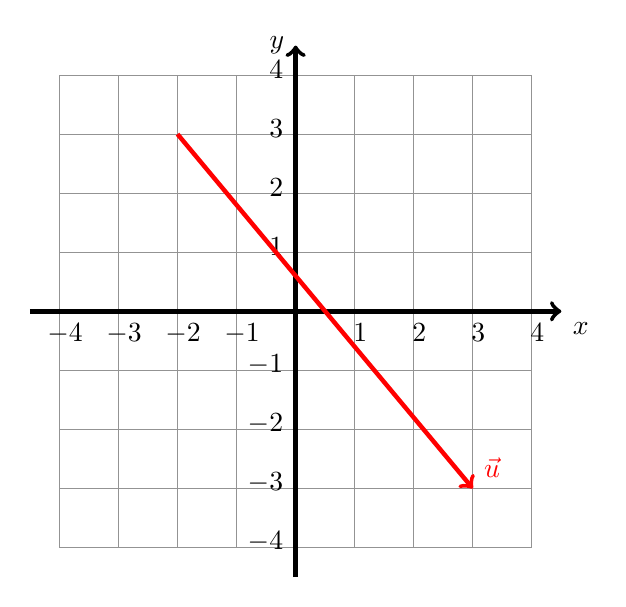
\begin{tikzpicture}[y=0.75cm, x=0.75cm,font=\sffamily]
        \draw[step = 1, gray, thin,opacity=0.85] (-4,-4) grid (4,4);
        \draw[black,ultra thick,->] (-4.5,0) -- (4.5,0) node[anchor=north west] {$x$};
        \draw[black,ultra thick,->] (0,-4.5) -- (0,4.5) node[anchor=east] {$y$};
        \foreach \y in {-4,-3,-2,-1,1,2,3,4} {
          \draw (1pt, \y) -- (-1pt, \y) node[anchor = east,yshift=2] {$\y$};
          \draw (\y,1pt) --  (\y,-1pt) node[anchor = north,xshift=2] {$\y$};
        }
        \draw[->,ultra thick,red] (-2,3)--(3,-3) node [anchor=south west]{$\vec{u}$};
      \end{tikzpicture}

  \end{columns}
\end{frame}

\begin{frame}{Vector as a coordinate}

  \begin{columns}
    \column{0.4\textwidth}
    if only one coordinate is given then it is assumed that the start
    point is at the origin.

    \uncover<2->{
      the vector that extends to $(3,-3)$.
      }

    \column<2->{0.6\textwidth}
    Example: Start and End Point Defining a Vector
      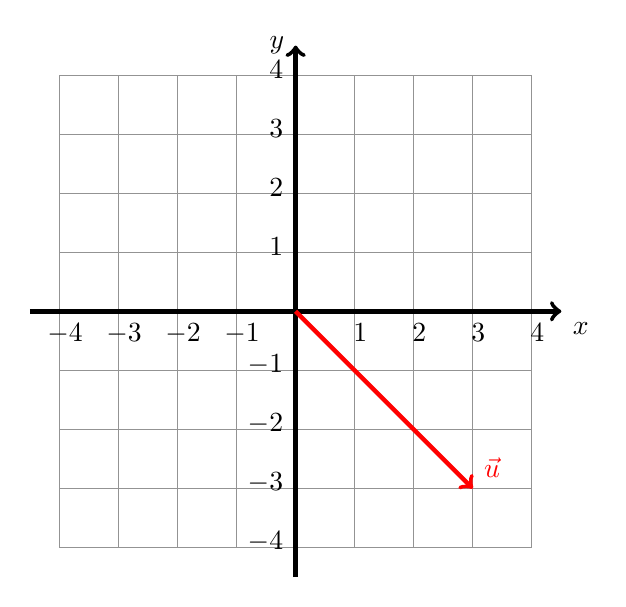
\begin{tikzpicture}[y=0.75cm, x=0.75cm,font=\sffamily]
        \draw[step = 1, gray, thin,opacity=0.85] (-4,-4) grid (4,4);
        \draw[black,ultra thick,->] (-4.5,0) -- (4.5,0) node[anchor=north west] {$x$};
        \draw[black,ultra thick,->] (0,-4.5) -- (0,4.5) node[anchor=east] {$y$};
        \foreach \y in {-4,-3,-2,-1,1,2,3,4} {
          \draw (1pt, \y) -- (-1pt, \y) node[anchor = east,yshift=2] {$\y$};
          \draw (\y,1pt) -- (\y,-1pt) node[anchor = north,xshift=2] {$\y$};
        }
        \draw[->,ultra thick,red] (0,0)--(3,-3) node [anchor=south west]{$\vec{u}$};
      \end{tikzpicture}

  \end{columns}
\end{frame}


\begin{frame}{Notation}

  There are many ways to denote a vector. You need to be flexible and
  alternate between the different representations.

  \begin{itemize}
  \item A vector of length $3\sqrt{2}$ that has an angle of
    $-45^\circ$ from the positive $x$-axis.
  \item The vector starting at $(0,0)$ and ends at $(3,-3)$.
  \item The vector that extends to $(3,-3)$.
  \item The vector $3\vec{\imath}-3\vec{\jmath}$.
  \item The vector $\columnVector{3 \\ -3}$.
  \end{itemize}
  All of these descriptions refer to the same vector. 
  
\end{frame}

\begin{frame}{More Notation}

  \begin{itemize}
  \item $\textbf{x}$
  \item $\vec{x}$
  \item $\hat{x}$
  \end{itemize}
  
\end{frame}

\section{Vector Operations}

\begin{frame}{Vector Operations}

  There are two basic operations you can do to a vector. These basic
  operations can be combined to make more complicated operations, but
  these are the basic building blocks.

  \begin{block}{Scalar Multiplication (Stretch/Compress)}
    If you multiply a vector by a scalar,
    \begin{eqnarray*}
      c\cdot \vec{x},
    \end{eqnarray*}
    you either stretch or
    compress the vector.
    \begin{itemize}
    \item If $|c|>1$ you stretch the vector.
    \item If $|c|<1$ you compress the vector.
    \item If $c$ is positive the result is in the same direction.
    \item If $c$ is negative you flip the direction of the vector.
    \end{itemize}
  \end{block}
  
\end{frame}

\begin{frame}{Example}

    \begin{columns}
      \column{0.4\textwidth}

      Compare the vector $\vec{u}=\columnVector{2 \\ -1}$ to
      $2\columnVector{2 \\ -1}$.

    \column{0.6\textwidth}
    Example: Start and End Point Defining a Vector
      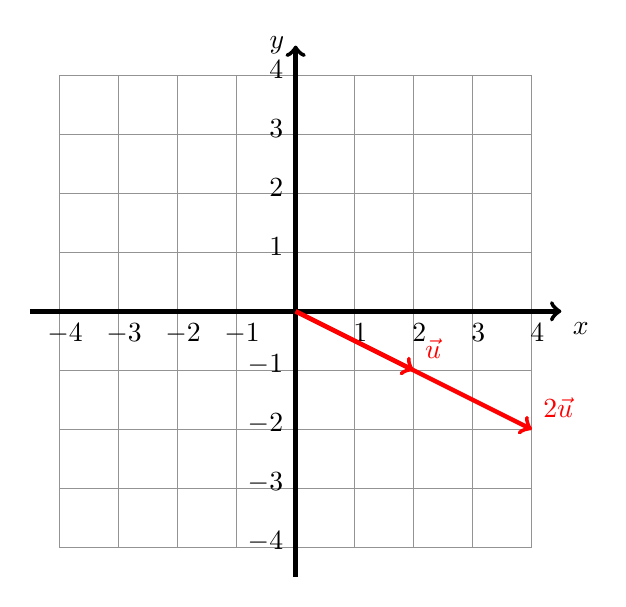
\begin{tikzpicture}[y=0.75cm, x=0.75cm,font=\sffamily]
        \draw[step = 1, gray, thin,opacity=0.85] (-4,-4) grid (4,4);
        \draw[black,ultra thick,->] (-4.5,0) -- (4.5,0) node[anchor=north west] {$x$};
        \draw[black,ultra thick,->] (0,-4.5) -- (0,4.5) node[anchor=east] {$y$};
        \foreach \y in {-4,-3,-2,-1,1,2,3,4} {
          \draw (1pt, \y) -- (-1pt, \y) node[anchor = east,yshift=2] {$\y$};
          \draw (\y,1pt) -- (\y,-1pt) node[anchor = north,xshift=2] {$\y$};
        }
        \draw<1>[->,ultra thick,red] (0,0)--(2,-1) node [anchor=south west]{$\vec{u}$};
        \draw<2>[->,ultra thick,red] (0,0)--(4,-2) node [anchor=south west]{$2\vec{u}$};
      \end{tikzpicture}

  \end{columns}

  
\end{frame}

\begin{frame}{Example}

    \begin{columns}
      \column{0.4\textwidth}

      Compare the vector $\vec{u}=\columnVector{2 \\ -1}$ to
      $-2\columnVector{2 \\ -1}$.

    \column{0.6\textwidth}
    Example: Start and End Point Defining a Vector
      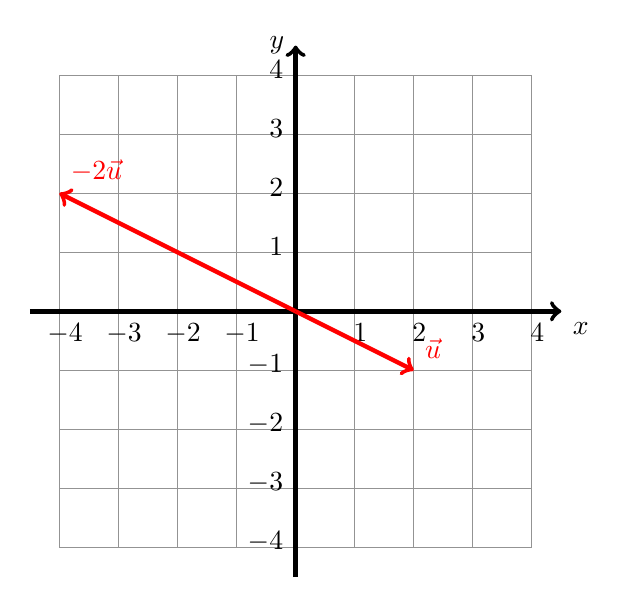
\begin{tikzpicture}[y=0.75cm, x=0.75cm,font=\sffamily]
        \draw[step = 1, gray, thin,opacity=0.85] (-4,-4) grid (4,4);
        \draw[black,ultra thick,->] (-4.5,0) -- (4.5,0) node[anchor=north west] {$x$};
        \draw[black,ultra thick,->] (0,-4.5) -- (0,4.5) node[anchor=east] {$y$};
        \foreach \y in {-4,-3,-2,-1,1,2,3,4} {
          \draw (1pt, \y) -- (-1pt, \y) node[anchor = east,yshift=2] {$\y$};
          \draw (\y,1pt) -- (\y,-1pt) node[anchor = north,xshift=2] {$\y$};
        }
        \draw<1>[->,ultra thick,red] (0,0)--(2,-1) node [anchor=south west]{$\vec{u}$};
        \draw<2>[->,ultra thick,red] (0,0)--(-4,2) node [anchor=south west]{$-2\vec{u}$};
      \end{tikzpicture}

  \end{columns}

  
\end{frame}

\begin{frame}{Example}

    \begin{columns}
      \column{0.4\textwidth}

      Compare the vector $\vec{u}=\columnVector{2 \\ -1}$ to
      $\frac{1}{2}\columnVector{2 \\ -1}$.

    \column{0.6\textwidth}
    Example: Start and End Point Defining a Vector
      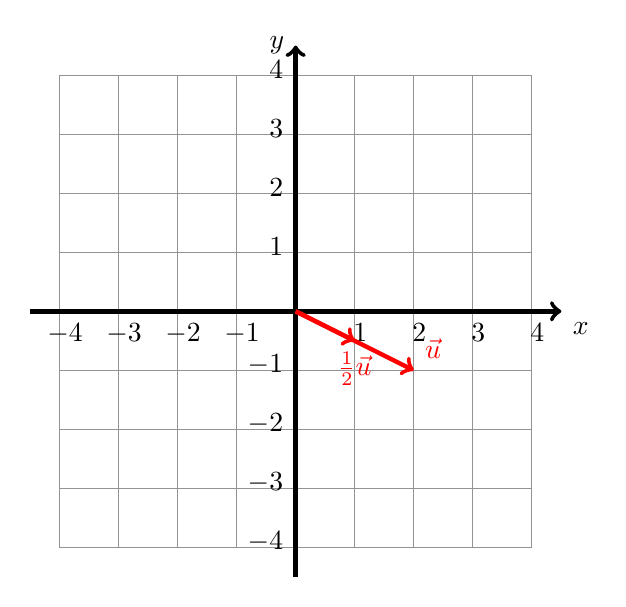
\begin{tikzpicture}[y=0.75cm, x=0.75cm,font=\sffamily]
        \draw[step = 1, gray, thin,opacity=0.85] (-4,-4) grid (4,4);
        \draw[black,ultra thick,->] (-4.5,0) -- (4.5,0) node[anchor=north west] {$x$};
        \draw[black,ultra thick,->] (0,-4.5) -- (0,4.5) node[anchor=east] {$y$};
        \foreach \y in {-4,-3,-2,-1,1,2,3,4} {
          \draw (1pt, \y) -- (-1pt, \y) node[anchor = east,yshift=2] {$\y$};
          \draw (\y,1pt) -- (\y,-1pt) node[anchor = north,xshift=2] {$\y$};
        }
        \draw<1>[->,ultra thick,red] (0,0)--(2,-1) node [anchor=south west]{$\vec{u}$};
        \draw<2>[->,ultra thick,red] (0,0)--(1,-0.5) node [anchor=north]{$\frac{1}{2}\vec{u}$};
      \end{tikzpicture}

  \end{columns}

  
\end{frame}

\begin{frame}{Example}

    \begin{columns}
      \column{0.4\textwidth}

      Compare the vector $\vec{u}=\columnVector{2 \\ -1}$ to
      $-\frac{1}{2}\columnVector{2 \\ -1}$.

    \column{0.6\textwidth}
    Example: Start and End Point Defining a Vector
      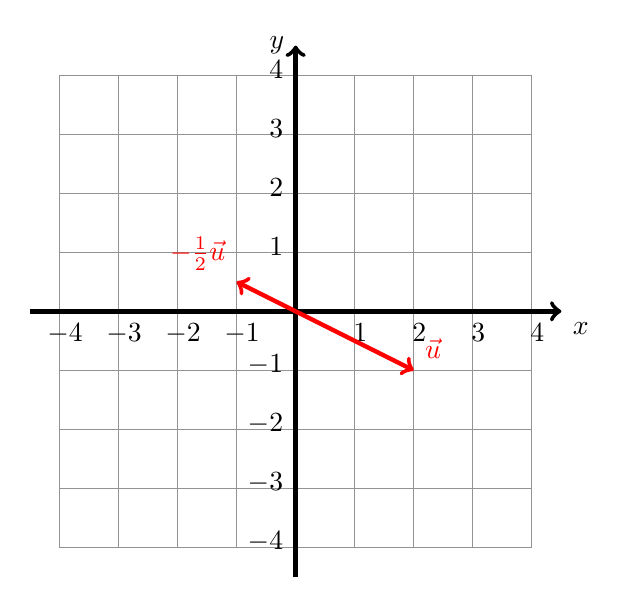
\begin{tikzpicture}[y=0.75cm, x=0.75cm,font=\sffamily]
        \draw[step = 1, gray, thin,opacity=0.85] (-4,-4) grid (4,4);
        \draw[black,ultra thick,->] (-4.5,0) -- (4.5,0) node[anchor=north west] {$x$};
        \draw[black,ultra thick,->] (0,-4.5) -- (0,4.5) node[anchor=east] {$y$};
        \foreach \y in {-4,-3,-2,-1,1,2,3,4} {
          \draw (1pt, \y) -- (-1pt, \y) node[anchor = east,yshift=2] {$\y$};
          \draw (\y,1pt) -- (\y,-1pt) node[anchor = north,xshift=2] {$\y$};
        }
        \draw<1>[->,ultra thick,red] (0,0)--(2,-1) node [anchor=south west]{$\vec{u}$};
        \draw<2>[->,ultra thick,red] (0,0)--(-1,0.5) node [anchor=south east]{$-\frac{1}{2}\vec{u}$};
      \end{tikzpicture}

  \end{columns}

  
\end{frame}


\begin{frame}{Vector Operations}

  The other basic operation is the sum of two vectors.

  \begin{block}{Vector Addition}
    To add two vectors you add the corresponding entries of the two vectors.
    \begin{eqnarray*}
      \columnVector{a \\ b} + \columnVector{c \\ d} & = &
      \columnVector{a+c \\ b+d}.
    \end{eqnarray*}
  \end{block}
  
\end{frame}


\begin{frame}{Graphical View}

      \begin{columns}
      \column{0.4\textwidth}

      Graphically we can think of this as ``stacking'' the two vectors
      head to tail.

    \column{0.6\textwidth}
    
      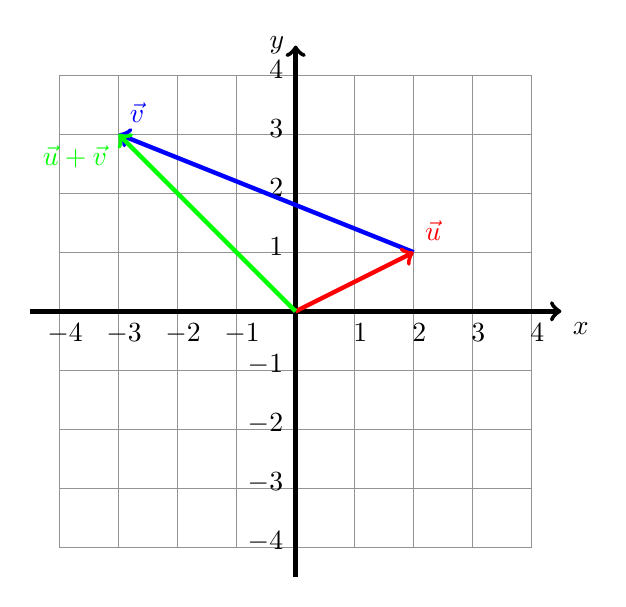
\begin{tikzpicture}[y=0.75cm, x=0.75cm,font=\sffamily]
        \draw[step = 1, gray, thin,opacity=0.85] (-4,-4) grid (4,4);
        \draw[black,ultra thick,->] (-4.5,0) -- (4.5,0) node[anchor=north west] {$x$};
        \draw[black,ultra thick,->] (0,-4.5) -- (0,4.5) node[anchor=east] {$y$};
        \foreach \y in {-4,-3,-2,-1,1,2,3,4} {
          \draw (1pt, \y) -- (-1pt, \y) node[anchor = east,yshift=2] {$\y$};
          \draw (\y,1pt) -- (\y,-1pt) node[anchor = north,xshift=2] {$\y$};
        }
        \draw[->,ultra thick,blue] (2,1)--(-3,3) node [anchor=south west]{$\vec{v}$};
        \draw[->,ultra thick,red] (0,0)--(2,1) node [anchor=south west]{$\vec{u}$};
        \draw<2->[->,ultra thick,green] (0,0)--(-3,3) node [anchor=north east]{$\vec{u}+\vec{v}$};
      \end{tikzpicture}

  \end{columns}
  
\end{frame}

\begin{frame}{Graphical View}

      \begin{columns}
      \column{0.4\textwidth}

      Graphically we can think of this as ``stacking'' the two vectors
      head to tail. Note that order does not matter.

      \column{0.6\textwidth}
    
      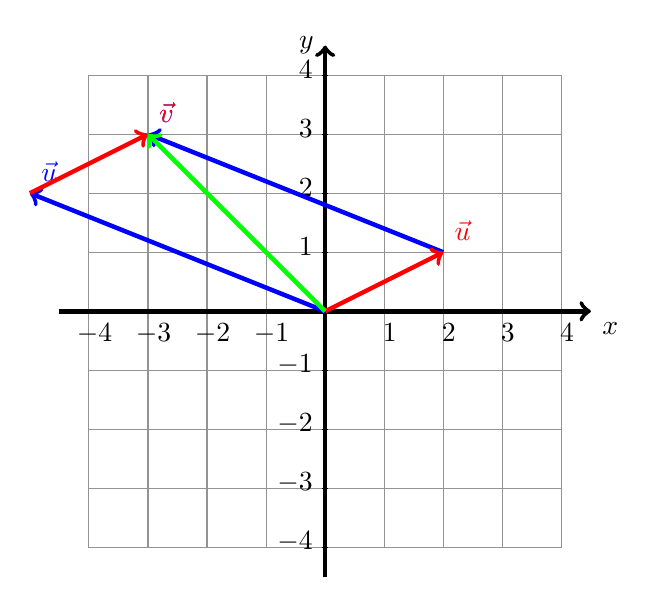
\begin{tikzpicture}[y=0.75cm, x=0.75cm,font=\sffamily]
        \draw[step = 1, gray, thin,opacity=0.85] (-4,-4) grid (4,4);
        \draw[black,ultra thick,->] (-4.5,0) -- (4.5,0) node[anchor=north west] {$x$};
        \draw[black,ultra thick,->] (0,-4.5) -- (0,4.5) node[anchor=east] {$y$};
        \foreach \y in {-4,-3,-2,-1,1,2,3,4} {
          \draw (1pt, \y) -- (-1pt, \y) node[anchor = east,yshift=2] {$\y$};
          \draw (\y,1pt) -- (\y,-1pt) node[anchor = north,xshift=2] {$\y$};
        }
        
        \draw[->,ultra thick,blue] (2,1)--(-3,3) node [anchor=south west]{$\vec{v}$};
        \draw[->,ultra thick,red] (0,0)--(2,1) node [anchor=south west]{$\vec{u}$};

        \draw[->,ultra thick,blue] (0,0)--(-5,2) node [anchor=south west]{$\vec{u}$};
        \draw[->,ultra thick,red] (-5,2)--(-3,3) node [anchor=south west]{$\vec{v}$};
        \draw<2->[->,ultra thick,green] (0,0)--(-3,3);
      \end{tikzpicture}

    \end{columns}

  \end{frame}

  \section{Linear Combinations of Vectors}

\begin{frame}{Combining The Two Operations}

  Now that we have two things, we can make a third by combining them.

  Example:
  \begin{eqnarray*}
    \vec{u} & = & \columnVector{2 \\ -1 }, \\
    \vec{v} & = & \columnVector{4 \\ 8}, \\
    3\vec{u} - \frac{1}{2} \vec{v} & = & 
  \end{eqnarray*}
    
\end{frame}

\begin{frame}{Combining The Two Operations}

  Example:
  \begin{eqnarray*}
    \vec{u} & = & \columnVector{2 \\ -1 }, \\
    \vec{v} & = & \columnVector{4 \\ 8}, \\
    \vec{u} -  \vec{v} & = & 
  \end{eqnarray*}
  (Vector Subtraction!)
    
\end{frame}

\begin{frame}{Combining The Two Operations}

  Example:
  \begin{eqnarray*}
    \vec{u} & = & \columnVector{2 \\ -1 }, \\
    \vec{v} & = & \columnVector{4 \\ 8}, \\
    7\vec{u} + 2\vec{v} & = & 
  \end{eqnarray*}
    
\end{frame}

\begin{frame}{Linear Combinations}

  Note that the sum of two vectors is a vector. That means we can add
  another vector to that result! We have essentially defined the
  addition of any number of vectors. Also, each one can be multiplied
  by a constant. There is literally no end to the joy we can have!

  \begin{block}{Defnition: Linear Combination of Vectors}

    If you are given a set of scalar values, $c_1$, $c_2$, $c_3$,
    $\ldots$, $c_k$ and a set of vectors, $\vec{u}_1$, $\vec{u}_2$,
    $\ldots$, $\vec{u}_k$, then a linear combination of the vectors is
    defined to be
    \begin{eqnarray*}
      c_1 \vec{u}_1 + c_2 \vec{u}_2 + c_3 \vec{u}_3 + \cdots + c_k \vec{u}_k.
    \end{eqnarray*}
    
  \end{block}
  
\end{frame}


\begin{frame}{Example: Linear Combination of Two Vectors}

  \begin{columns}
    \column{0.3\textwidth}

    \only<1>{
      \begin{eqnarray*}
        2\columnVector{1 \\ -2} + 3\columnVector{-2 \\ 1}
      \end{eqnarray*}
    }

    \only<2>{
      \begin{eqnarray*}
        c_1 \columnVector{1 \\ -2} + c_2 \columnVector{-2 \\ 1}
      \end{eqnarray*}
    }

    \column{0.7\textwidth}
  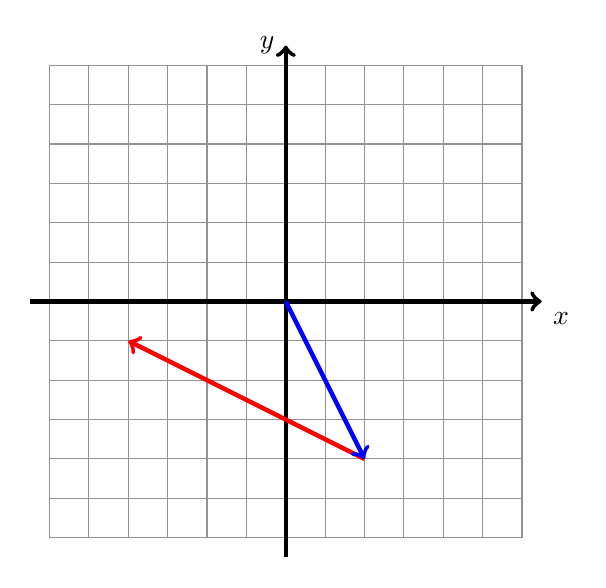
\begin{tikzpicture}[y=0.5cm, x=0.5cm,font=\sffamily]
    \draw[step = 1, gray, thin,opacity=0.85] (-6,-6) grid (6,6);
    \draw[black,ultra thick,->] (-6.5,0) -- (6.5,0) node[anchor=north west] {$x$};
    \draw[black,ultra thick,->](0,-6.5) -- (0,6.5) node[anchor=east] {$y$};

    \draw<1>[->,ultra thick,red] (2,-4)--(-4,-1);
    \draw<1>[->,ultra thick,blue] (0,0)--(2,-4);

  \end{tikzpicture}
  
\end{columns}
  
\end{frame}

\begin{frame}{Example: Linear Combination of Two Vectors}

  \begin{columns}
    \column{0.3\textwidth}

      \begin{eqnarray*}
        c_1 \columnVector{1 \\ -2} + c_2 \columnVector{2 \\ -4}
      \end{eqnarray*}


    \column{0.7\textwidth}
  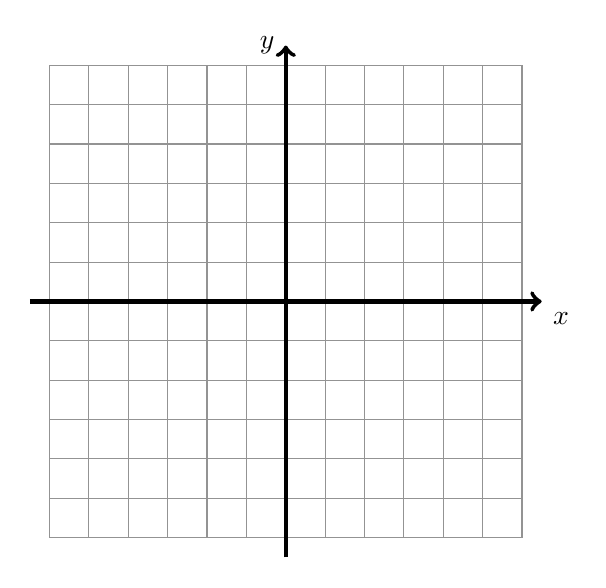
\begin{tikzpicture}[y=0.5cm, x=0.5cm,font=\sffamily]
    \draw[step = 1, gray, thin,opacity=0.85] (-6,-6) grid (6,6);
    \draw[black,ultra thick,->] (-6.5,0) -- (6.5,0) node[anchor=north west] {$x$};
    \draw[black,ultra thick,->](0,-6.5) -- (0,6.5) node[anchor=east] {$y$};

  \end{tikzpicture}
  
\end{columns}
  
\end{frame}


\begin{frame}{Blank Page}
  \dotfield{60}{24}
\end{frame}


\end{document}
